\section{LDPC Codes}
The LDPC codes, as the name suggests is characterized by a sparse parity check matrix \textbf{H}.
From parity check matrix we can construct the \textit{Tanner graph} of the code. For example
\cref{tanner_example} represents the Tanner graph of [7, 4, 3] Hamming code with
\begin{equation}
\label{H_matrix}
 \textbf{H} = 
 \left(
\begin{array}{ccccccc}
1 & 1 & 0 & 1 & 1 & 0 & 0  \\
1 & 0 & 1 & 1 & 0 & 1 & 0  \\
0 & 1 & 1 & 1 & 0 & 0 & 1 
\end{array}
\right)
\end{equation}
A codeword \textbf{x} from the codebook described by parity check matrix \textbf{H} should satisfy
\begin{equation}
\label{parity_check_equations}
 \textbf{H}\textbf{x} = \textbf{0}
\end{equation}
In the Tanner graph of a $(t_c, t_r)$ regular binary LDPC code, each variable node will have degree $t_c$ 
and each check node will have degree $t_r$. Irregular LDPC codes can have different degrees for nodes.
Let $\lambda$ and $\rho$ be vectors such that their $i^{th}$ component $\lambda_i$ and $\rho_i$ represent the fraction of edges
connecting to a variable node of degree $i$ and check node of degree $i$ respectively.
Thus
\begin{equation}\nonumber
\lambda(x) = \displaystyle \sum_i \lambda_ix^{i-1} \hspace{8pt}\text{and}\hspace{8pt} \rho(x) = \displaystyle \sum_i \rho_ix^{i-1}
\end{equation}
are called variable and check degree distribution polynomials respectively.
Standard ensemble LDPC$(n, \lambda, \rho)$ of bipartite graphs is defined as the set of bipartite graphs with
$n$ variable nodes, variable degree distribution $\lambda(x)$ and check degree distribution $\rho(x)$.
%===========================================================================================================================
\begin{figure}
\begin{center}
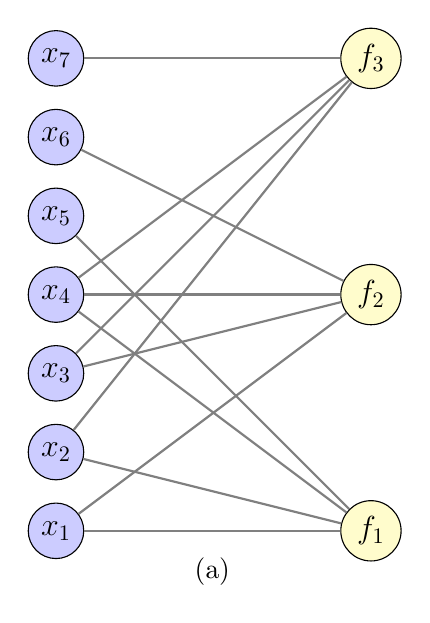
\begin{tikzpicture}[var node/.style={scale = 0.8, circle,fill=blue!20,draw,font=\sffamily\Large\bfseries}, fun node/.style={scale = 0.8, circle,fill=yellow!20,draw,font=\sffamily\Large\bfseries}]
  \node[var node] (x7) at (0, 0) {$x_7$};
  \node[var node] (x6) at (0, -1) {$x_6$};
  \node[var node] (x5) at (0, -2) {$x_5$};
  \node[var node] (x4) at (0, -3) {$x_4$};
  \node[var node] (x3) at (0, -4) {$x_3$};
  \node[var node] (x2) at (0, -5) {$x_2$};
  \node[var node] (x1) at (0, -6) {$x_1$};  
  \node[fun node] (f3) at (4, 0) {$f_3$};
  \node[fun node] (f2) at (4, -3) {$f_2$};
  \node[fun node] (f1) at (4, -6) {$f_1$};
  \draw[thick,draw=gray!100] (x1) -- node [below = 6pt] {(a)} (f1);
  \draw[thick,draw=gray!100] (x2) --  (f1);
  \draw[thick,draw=gray!100] (x4) --  (f1);
  \draw[thick,draw=gray!100] (x5) --  (f1);
  \draw[thick,draw=gray!100] (x1) --  (f2);
  \draw[thick,draw=gray!100] (x3) --  (f2);
  \draw[thick,draw=gray!100] (x4) --  (f2);
  \draw[thick,draw=gray!100] (x6) --  (f2);
  \draw[thick,draw=gray!100] (x3) --  (f3);
  \draw[thick,draw=gray!100] (x2) --  (f3);
  \draw[thick,draw=gray!100] (x4) --  (f3);
  \draw[thick,draw=gray!100] (x7) --  (f3);
\end{tikzpicture}
\caption{\scriptsize{Tanner graph of [7, 4, 3] Hamming code with \textbf{H} given in \cref{H_matrix}.
The blue nodes on the left represents the components of a codeword. They are called variable nodes.
The yellow nodes on the right represents each of the constraints in the system \cref{parity_check_equations}. They are called
check nodes. When $h_{i,j}$ is 1 there exists a link between $j^{th}$ variable node and $i^{th}$ check node.
}} 
\label{tanner_example}
\end{center}
\end{figure}